% Seminarski rad SREES — Azra Babic (19029)
% Otvoriti u LyX-u:  File -> Import -> LaTeX (plain)   (ili kompajlirati: pdflatex)
\documentclass[11pt,a4paper]{article}
\usepackage[utf8]{inputenc}
\usepackage[T1]{fontenc}
\usepackage{lmodern}
\usepackage[margin=2.5cm]{geometry}
\usepackage{amsmath,amssymb}
\usepackage{graphicx}
\usepackage{booktabs}
\usepackage{hyperref}
\usepackage{xcolor}

\title{\textbf{Konvertor nelinearnog strujnog balansa:\\ polarne koordinate}}
\author{Azra Babić, index 19029 \\ Predmet: SREES \\ natID SDK v4.1.0, dTwin 1.2.27}
\date{2026}

\begin{document}
\maketitle

\section{Uvod}
Proračun tokova snaga je osnovni proračun u elektroenergetskim sistemima: za zadane
injekcije snaga i topologiju mreže traže se naponi (moduli $V_i$ i uglovi $\delta_i$)
u svim čvorovima. Klasično se sistem formira preko \emph{balansa snaga} ($\Delta P$,
$\Delta Q$). Ovaj rad koristi ekvivalentnu formulaciju --- \emph{balans struja}
(engl.\ \textit{current injection / current balance}) u \textbf{polarnim koordinatama}.

Zadatak je \textbf{konvertor}: C++ plugin za framework \textbf{dTwin} koji iz opisa
mreže (MATPOWER \texttt{.m}) generiše tekstualni \texttt{.dmodl} NL model sa jednačinama
strujnog balansa. Model zatim rješava ugrađeni nelinearni rješavač dTwin-a
(Newton--Raphson). Konverzija radi u zasebnoj radnoj niti, dok se napredak prikazuje u
realnom vremenu na GUI niti; isporučuje se kao dinamička biblioteka (\texttt{dll}/\texttt{dylib})
koja se učitava u meniju \textbf{Model $\rightarrow$ Import}.

\section{Teorijska osnova}

\subsection{Matrica admitansi (Y-bus)}
Mreža se opisuje matricom admitansi $\mathbf{Y}$, uz vezu $\mathbf{I}=\mathbf{Y}\mathbf{V}$,
tj.\ $I_i=\sum_k Y_{ik}V_k$. Za granu $f$--$t$ sa serijskom admitansom $y=1/(r+jx)$,
otočnom $b_{sh}=j\,b/2$ i kompleksnim odnosom transformatora $a=t\,e^{j\varphi}$:
\[
Y_{ff}\!\mathrel{+}=\!\frac{y+b_{sh}}{a\,a^{*}},\quad
Y_{tt}\!\mathrel{+}=\!y+b_{sh},\quad
Y_{ft}\!\mathrel{+}=\!-\frac{y}{a^{*}},\quad
Y_{tf}\!\mathrel{+}=\!-\frac{y}{a}.
\]
Otočni elementi čvora $(G_s+jB_s)$ dodaju se na dijagonalu. U polarnom obliku
$Y_{ik}=Y_{ik}e^{j\theta_{ik}}$, $V_k=V_k e^{j\delta_k}$.

\subsection{Jednačine strujnog balansa}
Proračunata struja: $I_i^{calc}=\sum_k Y_{ik}V_k e^{j(\theta_{ik}+\delta_k)}$, pa je
\[
\Re\{I_i^{calc}\}=\sum_k Y_{ik}V_k\cos(\theta_{ik}+\delta_k),\qquad
\Im\{I_i^{calc}\}=\sum_k Y_{ik}V_k\sin(\theta_{ik}+\delta_k).
\]
Zadana struja iz $S_i=P_i+jQ_i=V_iI_i^{*}$ je $I_i^{sp}=\frac{P_i-jQ_i}{V_i}e^{j\delta_i}$,
odakle slijede jednačine balansa (dvije po čvoru):
\begin{align}
\sum_k Y_{ik}V_k\cos(\theta_{ik}+\delta_k) &= \frac{P_i\cos\delta_i+Q_i\sin\delta_i}{V_i},\\
\sum_k Y_{ik}V_k\sin(\theta_{ik}+\delta_k) &= \frac{P_i\sin\delta_i-Q_i\cos\delta_i}{V_i}.
\end{align}
Za razliku od balansa snaga
$\big(V_i\sum_k Y_{ik}V_k\cos(\delta_i-\theta_{ik}-\delta_k)=P_i\big)$, ovdje su rezidual
i Jakobijan izvedeni iz \textbf{struja}.

\subsection{Newton--Raphson i tipovi čvorova}
Sistem $\mathbf{f}(\mathbf{x})=\mathbf{0}$, $\mathbf{x}=[\delta,V]$, rješava se iterativno:
$\mathbf{J}\,\Delta\mathbf{x}=-\mathbf{f}$, $\mathbf{x}^{(\nu+1)}=\mathbf{x}^{(\nu)}+\Delta\mathbf{x}$,
gdje je $\mathbf{J}=\partial(\Delta I^{\Re},\Delta I^{\Im})/\partial(\delta,V)$ (rijedak).
Tipovi čvorova:
\begin{itemize}
  \item \textbf{Slack}: $V_i,\delta_i$ fiksni --- bez jednačina.
  \item \textbf{PQ}: zadani $P_i,Q_i$; nepoznate $\delta_i,V_i$.
  \item \textbf{PV}: zadani $P_i,|V_i|$; $V_i$ fiksan parametar, nepoznate $\delta_i$ i
        $Q_i^{g}$ (reaktivna injekcija).
\end{itemize}

\section{Implementacija}
Konvertor je \textbf{dTwin plugin} (\texttt{sc::IPlugin}). Tok:
\[
\text{MATPOWER .m}\;\rightarrow\;\text{Y-bus}\;\rightarrow\;\text{.dmodl}\;\rightarrow\;\text{dTwin NL solver}.
\]

\begin{figure}[h]\centering
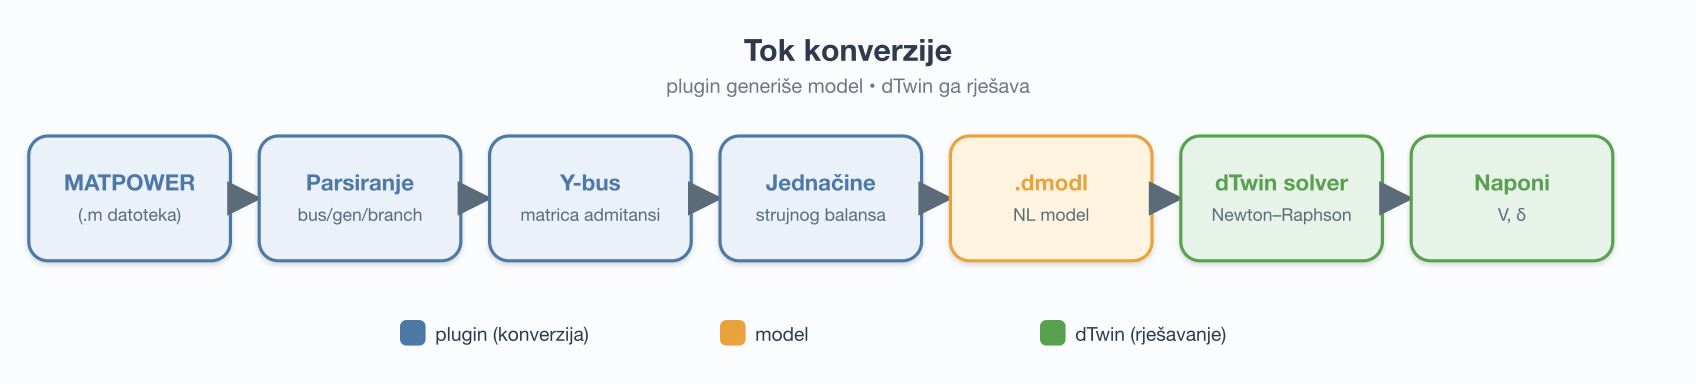
\includegraphics[width=\linewidth]{diagrams/02_tok_konverzije.png}
\caption{Tok konverzije: plugin generiše model, dTwin ga rješava.}
\end{figure}

\noindent\textbf{Struktura koda} (\texttt{src/CurrentBalancePlugin/}):
\texttt{Converter.h} (jezgra: parsiranje, Y-bus u natID \texttt{dense::CmplxMatrix}, generisanje \texttt{.dmodl}),
\texttt{CBPlugin.cpp} (IPlugin + \texttt{getPluginInterface}),
\texttt{WindowPlugin.h} (prozor), \texttt{ViewConv.h} (GUI + threading).

\paragraph{Generisane jednačine (primjer, PQ čvor 5).}
{\small
\begin{verbatim}
Y_5_5*V_5*cos(th_5_5+d_5)+... = (P_5*cos(d_5)+Q_5*sin(d_5))/V_5
Y_5_5*V_5*sin(th_5_5+d_5)+... = (P_5*sin(d_5)-Q_5*cos(d_5))/V_5
(u stvarnom modelu koriste se UTF-8 simboli th=theta, d=delta)
\end{verbatim}}

\paragraph{Višenitnost.} Konverzija se izvršava u radnoj niti (\texttt{std::thread}); GUI
ostaje responzivan, a progres-indikator se ažurira u realnom vremenu na glavnoj niti
(\texttt{gui::thread::asyncExecInMainThread}). Izlaz se piše preko \texttt{std::ofstream},
sadržaj se upisuje i u izlaznu arhivu.

\section{Rezultati i validacija}
Testni slučaj: MATPOWER \texttt{case9} (WSCC 9 čvorova, 3 generatora, 9 grana,
$S_{base}=100$~MVA).

\begin{figure}[h]\centering
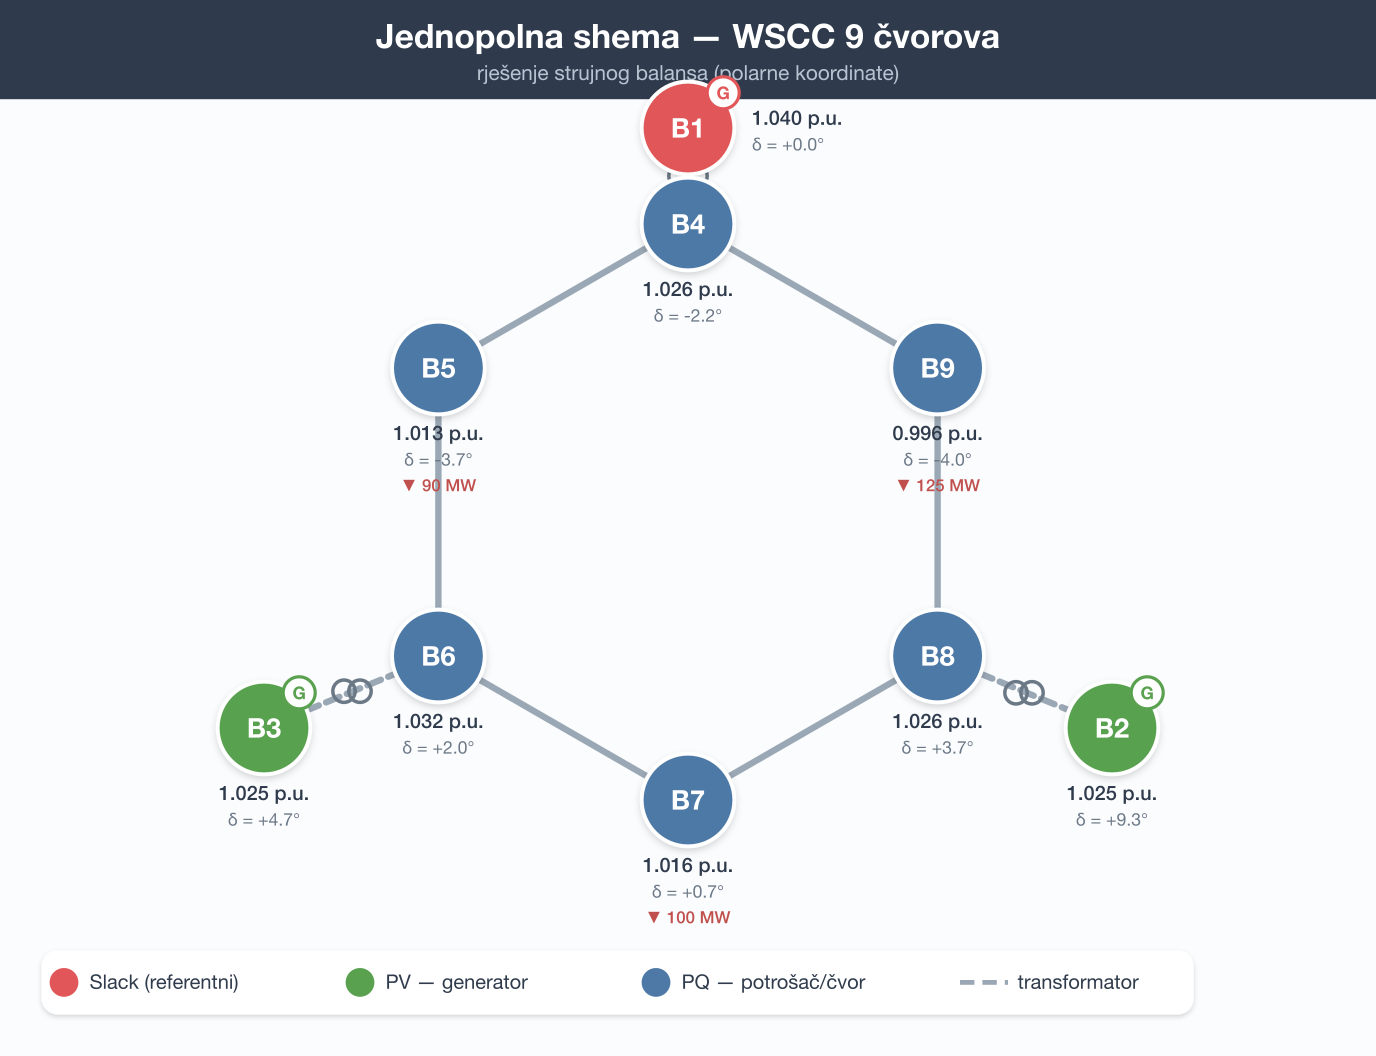
\includegraphics[width=0.78\linewidth]{diagrams/01_jednopolna_case9.png}
\caption{Jednopolna shema sa riješenim naponima (slack -- crveno, PV -- zeleno, PQ -- plavo).}
\end{figure}

Trostruka validacija:
\begin{enumerate}
  \item Y-bus se poklapa sa referentnim \texttt{case9.dmodl} do 10+ cifara.
  \item Reziduali jednačina strujnog balansa u tačnom rješenju: $2.4\cdot10^{-13}$;
        Newton--Raphson konvergira za 4 iteracije.
  \item Generisani model riješen dTwin-ovim \texttt{modSolver}-om: status \textbf{OK}.
\end{enumerate}

\begin{table}[h]\centering
\begin{tabular}{ccrr}
\toprule
Čvor & Tip & $V$ [p.u.] & $\delta$ [$^\circ$] \\
\midrule
1 & slack & 1.0400 & 0.00 \\
2 & PV & 1.0250 & 9.28 \\
3 & PV & 1.0250 & 4.67 \\
4 & PQ & 1.0258 & $-2.22$ \\
5 & PQ & 1.0127 & $-3.69$ \\
6 & PQ & 1.0324 & 1.97 \\
7 & PQ & 1.0159 & 0.73 \\
8 & PQ & 1.0258 & 3.72 \\
9 & PQ & 0.9956 & $-3.99$ \\
\bottomrule
\end{tabular}
\caption{Rješenje (dTwin modSolver). PV čvorovi: $Q_2^g=0.0665$, $Q_3^g=-0.1086$ p.u.}
\end{table}

\begin{figure}[h]\centering
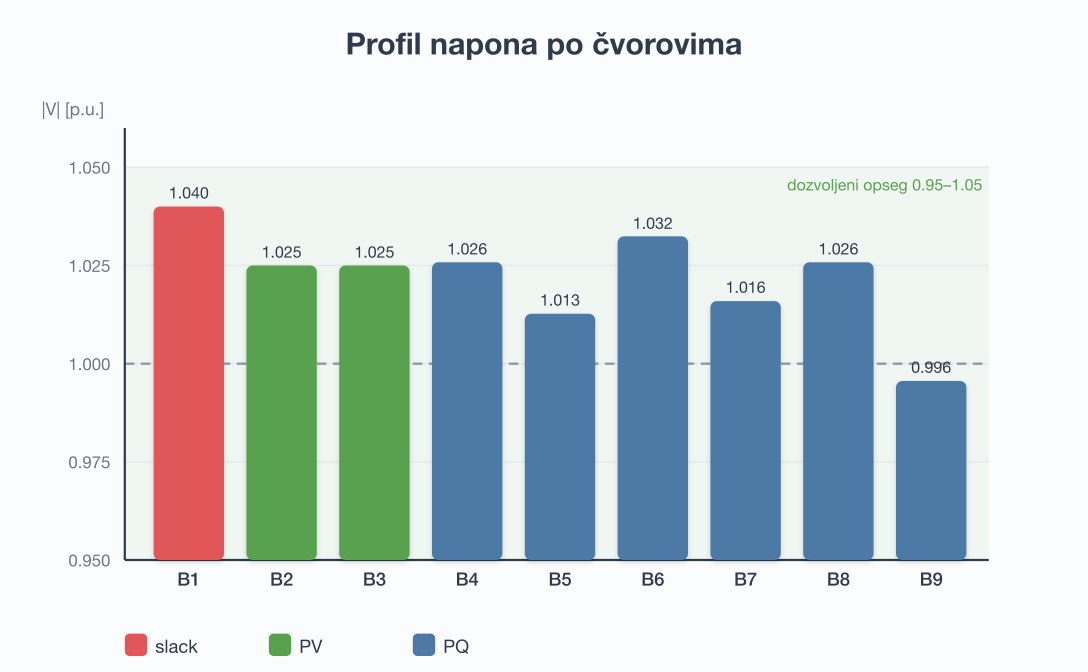
\includegraphics[width=0.6\linewidth]{diagrams/03_profil_napona.png}
\caption{Profil napona po čvorovima.}
\end{figure}

\section{Zaključak}
Implementiran je i validiran C++ plugin-konvertor koji generiše dTwin NL model tokova
snaga u formulaciji nelinearnog strujnog balansa u polarnim koordinatama. Analitički i
kroz stvarni dTwin rješavač pokazano je da formulacija daje fizički ispravno rješenje,
identično klasičnom balansu snaga. Ispunjeni su zahtjevi: C++, konverzija u zasebnoj
niti, real-time progres na drugoj (GUI) niti, GUI i isporuka kao plugin (\texttt{dll}).

\paragraph{Napomena o SDK-u.} Y-bus se gradi u natID kompleksnoj dense matrici
(\texttt{dense::CmplxMatrix}), a plugin koristi zvanični \texttt{arch/MemoryOut.h}. Ovi
headeri (\texttt{arch/MemoryOut.h}, \texttt{matrix/MatrixLib.h}) nedostajali su u ranijem
release-u (v4.1.0), ali su prisutni u aktuelnoj \emph{main grani} natID-a, pa build zahtijeva
tu (ili noviju) verziju SDK-a.

\begin{thebibliography}{9}
\bibitem{kundur} P.\ Kundur, \emph{Power System Stability and Control}, McGraw-Hill, 1994.
\bibitem{sauer} P.\ W.\ Sauer, M.\ A.\ Pai, \emph{Power System Dynamics and Stability}, 2007.
\bibitem{milano} F.\ Milano, \emph{Power System Modelling and Scripting}, Springer, 2010.
\bibitem{cim} V.\ M.\ da Costa et al., ``Power Flow Based on Current Injections'',
  \emph{IEEE Trans.\ Power Systems}, 1999.
\bibitem{matpower} R.\ D.\ Zimmerman et al., \emph{MATPOWER}.
\bibitem{natid} I.\ Džafić, \emph{natID} i \emph{dTwin} (github.com/idzafic).
\end{thebibliography}

\end{document}
